% 2011 年陕西卷文科第 15B 题：四边形 ABCD 与 AD、BC 的交点 E。
% 来源 PDF：普通高考/2011/2011陕西文.pdf，SHA-256 ae7984faa1d48b19525f0991a1795d8ea34b7ac65d9c067f4862c59ae112880e。
% 原页：第 1 页第 3 栏中部，书页码 695。
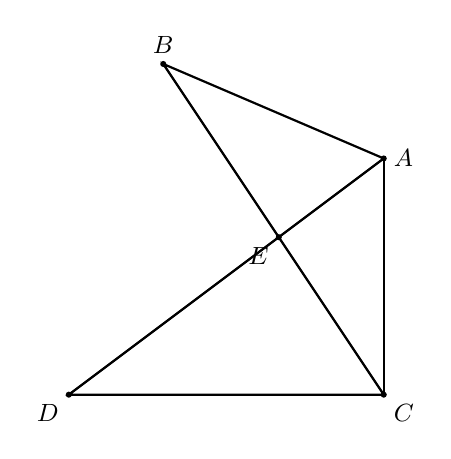
\begin{tikzpicture}[>=stealth, semithick, font=\small, scale=1.0]
  \coordinate (D) at (0,0);
  \coordinate (C) at (4,0);
  \coordinate (A) at (4,3);
  \coordinate (B) at (1.2,4.2);
  \coordinate (E) at (2.667,2.0);
  \draw[thick] (C)--(D)--(A)--(B)--(C);
  \draw[thick] (A)--(C);
  \draw (B)--(E)--(C);
  \draw (A)--(E)--(D);
  \fill (A) circle (1.1pt) node[right] {$A$};
  \fill (B) circle (1.1pt) node[above] {$B$};
  \fill (C) circle (1.1pt) node[below right] {$C$};
  \fill (D) circle (1.1pt) node[below left] {$D$};
  \fill (E) circle (1.1pt) node[below left] {$E$};
\end{tikzpicture}
